\chapter{Schemes}

\section{BLISS Software Implementation}

\subsection{Introduction}
The emphasis (at this stage) of the library is to create a flexible software library on which various lattice-based cryptographic schemes can be developed and implemented to a level of production quality. It is a requirement that the library is highly portable and used as a research and development tool, therefore highly optimized inline assembly and extracting every cycle of performance are not the goals, but are possible. It is a requirement that confidence in \textit{libsafecrypto} is achieved by using thorough testing of the software (unit testing, functional testing and known-answer tests) together with a build system that integrates this testing into its build process. Also, where cryptographic primitives are required they will be drawn from well-established and well-respected implementations in the public domain.

The first algorithm to be implemented with the \textit{libsafecrypto} library is BLISS, which is a lattice-based digital signature scheme based on the Ring-LWE problem. The BLISS software implementation is originally based on the hilabliss \url{(https://github.com/mjosaarinen/hilabliss)} and BLZZRD (\url{https://github.com/mjosaarinen/blzzrd}) implementations created by Markku-Juhani O. Saarinen. This in turn is based on the BLISS-B variant of BLISS \url{(https://eprint.iacr.org/2014/874}) by Léo Ducas, derived from the original paper \url{(https://eprint.iacr.org/2013/383)}.

\subsection{Key Generation}

\begin{itemize}
\item $f$, $g$ are uniform random polynomials with a specific number of $\pm 1$ and $\pm 2$ coefficients
\item $g = 2g + 1$
\item $a = g / f$, if $f$ is not invertible then \textbf{Restart}.
\end{itemize}

In summary, the private key $(f, g)$ and public key $a$ are generated. In a practical implementation the following is also performed:

\begin{itemize}
\item To save cycles the public key is stored and distributed in the NTT domain. This saves 1 NTT in the signature and verification schemes. \textbf{What if someone finds something better than the NTT?}
\item The sign of $g$ must be inverted \textbf{(WHY???)}. From the hilabliss/BLZZRD original this is done by INTT, sign inversion, followed by NTT. The same can be achieved by simply performing the sign inversion in the NTT domain - giving an approx. 25\% boost in performance by saving a single NTT and INTT. I think this should be regarded as a bug fix rather than an optimisation
\item The two private keys are sparse polynomials and are ripe for compression, whereas the public key is randomly distributed across the range of the modulus and lossless compression tends to make it bigger. Note that the $g$ polynomial contains only the coefficients $\pm 2$ and $\pm 4$ with the exception of the first coefficient - this is exploited by all of the entropy coders. 
\end{itemize}

\subsection{Signatures}

\begin{itemize}
\item Generate $y_1$ and $y_2$ using a Gaussian sampler.
\item $u = y_1 * a + y_2 \bmod 2q$
\item $c = H(\lfloor u \rceil_d \bmod p, \mu)$
\item Choose a random bit $b$
\item $z_1 = y_1 + (-1)^b s_1 c$
\item $z_2 = y_2 + (-1)^b s_2 c$
\item \textbf{Continue} if a randomly chosen value between 0.0 and 1.0 is greater than a rejection threshold computed using a parameter set factor $M$  and the scalar product of the polynomials $s$, $c$, $y_1$ and $y_2$. Otherwise \textbf{Restart}.
\item $z_2 = ( \lfloor u \rceil_d - \lfloor u - z_2 \rceil_d \bmod p$
\item \textbf{Output} $(z_1, z_2, c)$
\end{itemize}

The main bottlenecks in this operation are the NTT/INTT, the hash function \textit{H()} and of course the rejection sampling which causes the signature to retry with a probability associated with the parameter set variables (e.g. 1.6 with BLISS-B-IV). To overcome these performance issues the following measures have been taken:

\subsubsection{Hash Functions}

\begin{itemize}
\item We've provided a choice of hashing function's that offer different performance and security properties (SHA-2 \cite{sha2_gladman}, SHA-3 \cite{tiny_sha3}, Whirlpool \cite{whirlpool} and BLAKE2-B \cite{blake2}). Currently it is fixed to SHA3-512, but this can be overridden with the relevant flags passed to the \textit{create()} function. The security of the hash must be relative to the security of the signature scheme, therefore there is a possibility that we can use smaller hash blocks with lower security parameter sets rather than the 512-bit message digest that is used by default with all parameter sets.
\begin{itemize}
  \item BLAKE2-B and SHA2 offer much better performance than SHA3, with Whirlpool not far behind (see Figure \ref{fig:bliss_b_hash_comparison}).

\pgfplotsset{compat=1.13,width=14cm,height=12cm}
\begin{figure}[ht!]
\centering
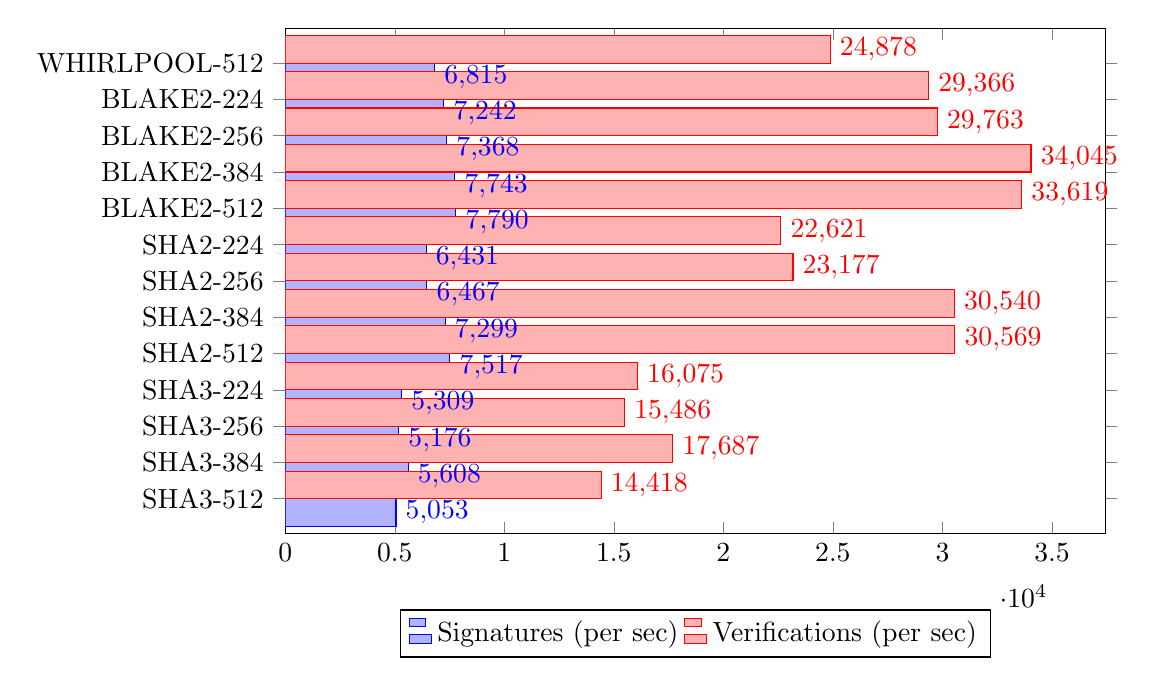
\begin{tikzpicture}
\begin{axis}[xbar=0pt, xmin=0, ytick=data, enlarge y limits=0.08, symbolic y coords={SHA3-512, SHA3-384, SHA3-256, SHA3-224, SHA2-512, SHA2-384, SHA2-256, SHA2-224, BLAKE2-512, BLAKE2-384, BLAKE2-256, BLAKE2-224, WHIRLPOOL-512}, y tick label style={/pgf/number format/1000 sep=}, nodes near coords, nodes near coords align={horizontal}, legend style={at={(0.5,-0.15)},anchor=north,legend columns=-1}]
\addplot
  coordinates
    {(5053,SHA3-512) (5608,SHA3-384) (5176,SHA3-256) (5309,SHA3-224)
     (7517,SHA2-512) (7299,SHA2-384) (6467,SHA2-256) (6431,SHA2-224)
     (7790,BLAKE2-512) (7743,BLAKE2-384) (7368,BLAKE2-256) (7242,BLAKE2-224)
     (6815,WHIRLPOOL-512)};

\addplot
  coordinates
    {(14418,SHA3-512) (17687,SHA3-384) (15486,SHA3-256) (16075,SHA3-224)
     (30569,SHA2-512) (30540,SHA2-384) (23177,SHA2-256) (22621,SHA2-224)
     (33619,BLAKE2-512) (34045,BLAKE2-384) (29763,BLAKE2-256) (29366,BLAKE2-224)
     (24878,WHIRLPOOL-512)};
\legend{Signatures (per sec), Verifications (per sec)}
\end{axis}
\end{tikzpicture}
\caption{BLISS-B-IV performance with various hash functions (Intel i7 6700 CPU @ 3.4GHz)}
\label{fig:bliss_b_hash_comparison}
\end{figure}

  \item BLAKE2-B lost out to Keccak in the SHA3 NIST competition, but it is an RFC (7693, draft).

\end{itemize}
\item A standalone performance analysis of the various hashing functions integrated into \textit{libsafecrypto} is provided in Figure \ref{fig:bliss_b_bytes_per_sec}:
\end{itemize}


\pgfplotsset{compat=1.13,width=14cm,height=22cm}
\begin{figure}[ht!]
\centering
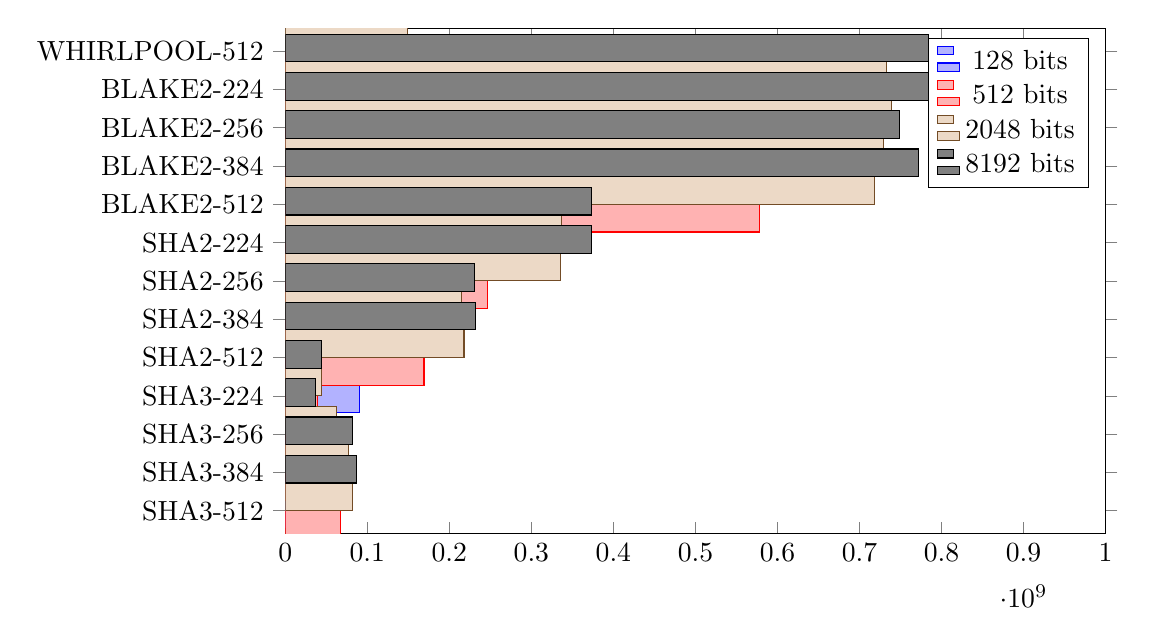
\begin{tikzpicture}
\begin{axis}[xbar=0pt, xmin=0, xmax=1000000000, ytick=data, enlarge y limits=0.05, symbolic y coords={SHA3-512, SHA3-384, SHA3-256, SHA3-224, SHA2-512, SHA2-384, SHA2-256, SHA2-224, BLAKE2-512, BLAKE2-384, BLAKE2-256, BLAKE2-224, WHIRLPOOL-512}, y tick label style={/pgf/number format/1000 sep=}]
\addplot
  coordinates
    {(41733600,SHA3-512) (66453490,SHA3-384) (33580860,SHA3-256) (26117498,SHA3-224) (90001193,SHA2-512) (111962015,SHA2-384) (137634227,SHA2-256) (133880238,SHA2-224) (318378956,BLAKE2-512) (245563664,BLAKE2-384) (143380969,BLAKE2-256) (341531003,BLAKE2-224) (63398434,WHIRLPOOL-512)};
\addplot
  coordinates
    {(67311617,SHA3-512) (47430787,SHA3-384) (60777654,SHA3-256) (39262358,SHA3-224) (169106491,SHA2-512) (176718677,SHA2-384) (246871771,SHA2-256) (250791574,SHA2-224) (577727014,BLAKE2-512) (582344548,BLAKE2-384) (589684613,BLAKE2-256) (591718794,BLAKE2-224) (131113251,WHIRLPOOL-512)};
\addplot
  coordinates
    {(81599679,SHA3-512) (76776751,SHA3-384) (62408720,SHA3-256) (43766790,SHA3-224) (217818471,SHA2-512) (214763352,SHA2-384) (335508930,SHA2-256) (336483310,SHA2-224) (718552357,BLAKE2-512) (729769587,BLAKE2-384) (738456684,BLAKE2-256) (732518714,BLAKE2-224) (149474568,WHIRLPOOL-512)};
\addplot
  coordinates
    {(87154415,SHA3-512) (81770554,SHA3-384) (36837864,SHA3-256) (44490799,SHA3-224) (231389170,SHA2-512) (230322287,SHA2-384) (372942248,SHA2-256) (373587750,SHA2-224) (771918396,BLAKE2-512) (748316921,BLAKE2-384) (788611685,BLAKE2-256) (783909562,BLAKE2-224) (158717452,WHIRLPOOL-512)};
\legend{128 bits, 512 bits, 2048 bits, 8192 bits}
\end{axis}
\end{tikzpicture}
\caption{Bytes per second performance of hash functions with varying message lengths [Intel i7 6700 CPU @ 3.4GHz]}
\label{fig:bliss_b_bytes_per_sec}
\end{figure}

\begin{itemize}
\item Profiling of the functional test executable for BLISS-B in \textit{valgrind/kcachegrind} shows that the performance bottlenecks are principally the hash function and the NTT, therefore small improvements to the associated functions provide reasonable performance gains.

\begin{itemize}

  \item Markku's Keccak/SHA3 has been optimised with some measures to manually perform loop unrolling so that the compiler doesn't have to use high (and potentially unstable) optimisation levels to achieve the same level of loop unrolling. However, this will be at the cost of an increased image size.

\begin{verbatim}
#ifdef SHA3_UNROLLED
    bc[0] = st[0] ^ st[0 + 5] ^ st[0 + 10] ^ st[0 + 15] ^ st[0 + 20];
    bc[1] = st[1] ^ st[1 + 5] ^ st[1 + 10] ^ st[1 + 15] ^ st[1 + 20];
    bc[2] = st[2] ^ st[2 + 5] ^ st[2 + 10] ^ st[2 + 15] ^ st[2 + 20];
    bc[3] = st[3] ^ st[3 + 5] ^ st[3 + 10] ^ st[3 + 15] ^ st[3 + 20];
    bc[4] = st[4] ^ st[4 + 5] ^ st[4 + 10] ^ st[4 + 15] ^ st[4 + 20];
#else
    for (i = 0; i < 5; i++) {
        bc[i] = st[i] ^ st[i + 5] ^ st[i + 10] ^ st[i + 15] ^ st[i + 20];
    }
#endif
\end{verbatim}

  \item Small indexing calculations in SHA-3 that are used repeatedly in loops where providing a large latency, therefore this has been replaced with 5 small LUTs to store the precomputed values.

\begin{verbatim}
    int i4mod5[5] = {4, 0, 1, 2, 3};
    int i1mod5[5] = {1, 2, 3, 4, 0};

    ...

    for (i = 0; i < 5; i++) {
        t = bc[i4mod5[i]] ^ ROTL64(bc[i1mod5[i]], 1);
        for (j = 0; j < 25; j += 5) {
            st[j + i] ^= t;
        }
    }
\end{verbatim}

As opposed to the original:

\begin{verbatim}
    for (i = 0; i < 5; i++) {
        t = bc[(i + 4) % 5] ^ ROTL64(bc[(i + 1) % 5], 1);
        for (j = 0; j < 25; j += 5) {
            st[j + i] ^= t;
        }
    }
\end{verbatim}
\end{itemize}
\end{itemize}


\clearpage
\subsubsection{Signature Restart}
\begin{itemize}
\item To improve the performance of the \textbf{Restart} if the rejection threshold is not met we have implemented a cheap but effective trick - every other time the signature algorithm is restarted the two random polynomials (sampled from a Gaussian distribution in the previous iteration) are simply swapped rather than re-generated, gaining approx. 10\%-25\% more signatures per second as shown in Figure \ref{fig:bliss_b_gaussian_swapping}.

\pgfplotsset{compat=1.13,width=15cm,height=7cm}
\begin{figure}[ht!]
\centering
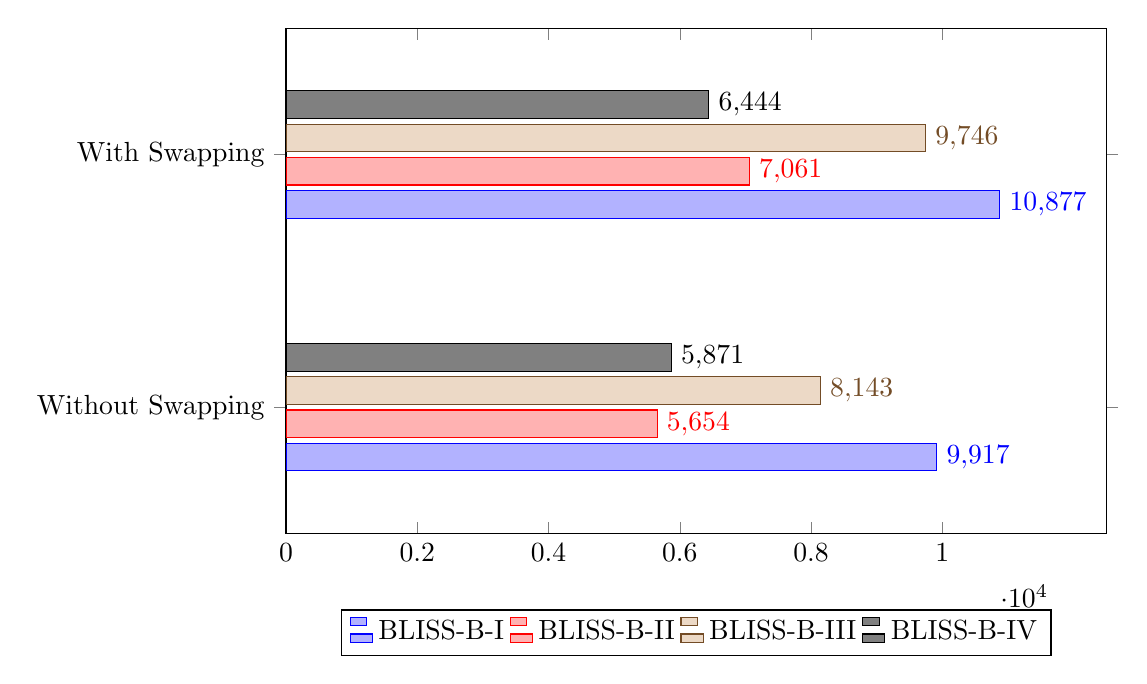
\begin{tikzpicture}
\begin{axis}[xbar, xmin=0, xmax=12500, xtick={0,2000,4000,6000,8000,10000}, ytick=data, enlarge y limits=0.5, symbolic y coords={Without Swapping, With Swapping}, y tick label style={/pgf/number format/1000 sep=}, nodes near coords, nodes near coords align={horizontal}, legend style={at={(0.5,-0.15)},anchor=north,legend columns=-1},]
\addplot coordinates {(9917,Without Swapping) (10877,With Swapping)};
\addplot coordinates {(5654,Without Swapping) (7061,With Swapping)};
\addplot coordinates {(8143,Without Swapping) (9746,With Swapping)};
\addplot coordinates {(5871,Without Swapping) (6444,With Swapping)};
\legend{BLISS-B-I, BLISS-B-II, BLISS-B-III, BLISS-B-IV}
\end{axis}
\end{tikzpicture}
\caption{Signatures per second performance of BLISS-B with no entropy coding and Restarts with/without Gaussian swapping [Intel i7 6700 CPU @ 3.4GHz]}
\label{fig:bliss_b_gaussian_swapping}
\end{figure}

\begin{itemize}
  \item In other schemes with a retrial a similar technique could be used. As BLISS must generate two Gaussian distributions it can quickly swap memory pointers rather than swapping the actual memory contents. Other schemes with only a single Gaussian distribution could employ methods to filter, scramble or partially update the existing distribution rather than create an entirely new polynomial using a Gaussian sampler.
\end{itemize}
\end{itemize}

\subsubsection{Entropy Coding}
\begin{itemize}
\item The signature is composed of three polynomials, $z_1$, $z_2$ and $c$. $z_1$ is a 12-bit code with a Gaussian distribution which can be exploited with an entropy coder to reduce the signature size. $z_2$ is a 2, 3 or 4 bit sparse polynomial (depending on the parameter set selected) that can also be readily compressed. The third polynomial $c$ contains random indices for an $n$ element polynomial and is short in length (12 to 39 elements) and therefore compression gains are minimal. The performance of BLISS-B signature compression is seen in Figure \ref{fig:bliss_b_signature_compression}, whilst the performance of the various entropy coders is shown in Figure \ref{fig:bliss_b_signature_compression_performance}.

\pgfplotsset{compat=1.13,width=14cm,height=8cm}
\begin{figure}[ht!]
\centering
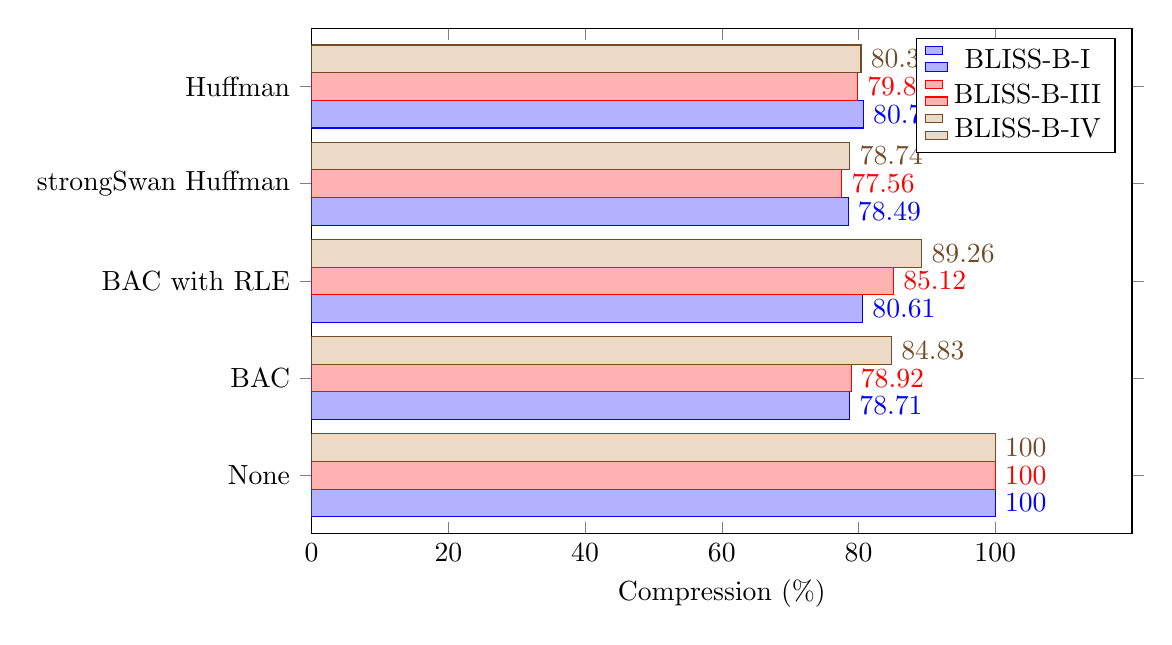
\begin{tikzpicture}
\begin{axis}[xbar=0pt, xlabel=Compression (\%), xmin=0, xmax=120, xtick={0,20,40,60,80,100}, ytick=data, enlarge y limits=0.15, symbolic y coords={None, BAC, BAC with RLE, strongSwan Huffman, Huffman}, y tick label style={/pgf/number format/1000 sep=}, nodes near coords, nodes near coords align={horizontal}]
\addplot coordinates {(100,None) (78.709,BAC) (80.606,BAC with RLE) (78.487,strongSwan Huffman) (80.721,Huffman)};
\addplot coordinates {(100,None) (78.918,BAC) (85.116,BAC with RLE) (77.555,strongSwan Huffman) (79.869,Huffman)};
\addplot coordinates {(100,None) (84.829,BAC) (89.264,BAC with RLE) (78.737,strongSwan Huffman) (80.36,Huffman)};
\legend{BLISS-B-I, BLISS-B-III, BLISS-B-IV}
\end{axis}
\end{tikzpicture}
\caption{BLISS-B Signature Compression with various entropy coders}
\label{fig:bliss_b_signature_compression}
\end{figure}

\pgfplotsset{compat=1.13,width=14cm,height=8cm}
\begin{figure}[ht!]
\centering
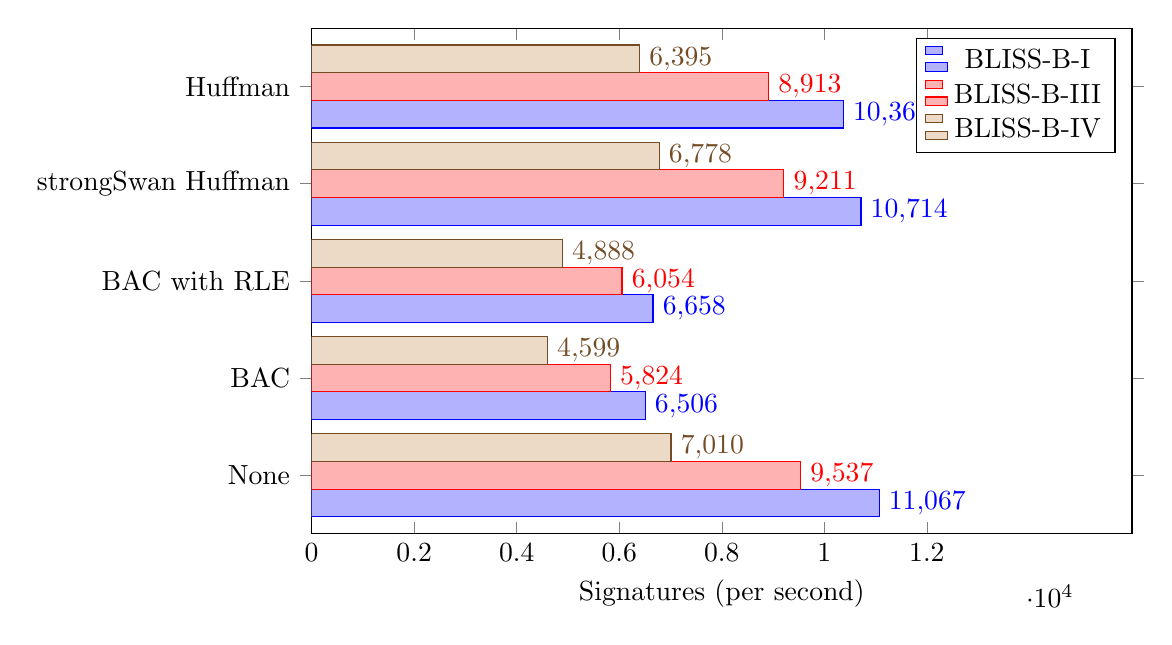
\begin{tikzpicture}
\begin{axis}[xbar=0pt, xlabel=Signatures (per second), xmin=0, xmax=16000, xtick={0,2000,4000,6000,8000,10000,12000}, ytick=data, enlarge y limits=0.15, symbolic y coords={None, BAC, BAC with RLE, strongSwan Huffman, Huffman}, y tick label style={/pgf/number format/1000 sep=}, nodes near coords, nodes near coords align={horizontal}]
\addplot coordinates {(11067,None) (6506,BAC) (6658,BAC with RLE) (10714,strongSwan Huffman) (10369,Huffman)};
\addplot coordinates {(9537,None) (5824,BAC) (6054,BAC with RLE) (9211,strongSwan Huffman) (8913,Huffman)};
\addplot coordinates {(7010,None) (4599,BAC) (4888,BAC with RLE) (6778,strongSwan Huffman) (6395,Huffman)};
\legend{BLISS-B-I, BLISS-B-III, BLISS-B-IV}
\end{axis}
\end{tikzpicture}
\caption{Performance of BLISS-B Signature Compression with various entropy coders [Intel i7 6700 CPU @ 3.4GHz]}
\label{fig:bliss_b_signature_compression_performance}
\end{figure}

\item The norms of the signature are currently checked by the signature algorithm, however this is not required and can be removed for a small performance gain.
\end{itemize}

\clearpage
\subsubsection{NTT/INTT}
\begin{itemize}

  \item The NTT loops have been modified to reduce some loop overhead in generating control variables, where possible they've been modified to encourage the compiler to use loop vectorisation and SIMD instructions.
  \item The NTT being used requires bit shuffling. This requires a function to swap each element of the polynomial with the element indexed by the bit reverse of it's index (\textit{see inverse\_shuffle\_32() in ntt.c}). For example, ARM instruction sets have a bit reverse instruction that can readily obtain the correct index for the swap operation.

\begin{verbatim}

UINT32 sc_bit_reverse_32(UINT32 x)
{
#ifdef __arm__
    UINT32 y;
    __asm__("rbit %0, %1\n" : "=r"(y) : "r"(x));
    return y;
#else
    x = (((x & 0xaaaaaaaa) >> 1) | ((x & 0x55555555) << 1)); // Swap odd and even
    x = (((x & 0xcccccccc) >> 2) | ((x & 0x33333333) << 2)); // Swap pairs
    x = (((x & 0xf0f0f0f0) >> 4) | ((x & 0x0f0f0f0f) << 4)); // Swap nibbles
    x = (((x & 0xff00ff00) >> 8) | ((x & 0x00ff00ff) << 8)); // Swap bytes
    return (x >> 16) | (x << 16);                            // Swap pairs of bytes
#endif
}

...

// Make use of a bit reversal instruction
UINT32 bits = 32 - sc_ctz_32(n);
for (i = 1; i < n-1; i++) {       // 00..0 and 11..1 remain same
    UINT32 r = sc_bit_reverse_32(i);
    r >>= bits;
    if (i < r) {
        SINT32 x = v[i];
        v[i] = v[r];
        v[r] = x;
    }
}
\end{verbatim}

  \item On x86 we can use the gcc \textit{builtin\_ctz} function (if available) to provide a more optimal bit reversal function by incrementing the MSB's to obtain bit reversal.

\begin{verbatim}
// If a BUILTIN funtion exists for CTZ then inverse incremental
// counting can be achieved by incrementing the MSB's
UINT32 bits = sc_ctz_32(n) - 1;
j = n >> 1;
for (i = 1; i < n - 1;) {       // 00..0 and 11..1 remain same
    if (i < j) {
        SINT32 x = v[i];
        v[i] = v[j];
        v[j] = x;
    }
    UINT32 mask = i++;
    mask ^= i;
    UINT32 len = sc_ctz_32(i);
    mask <<= bits - len;
    j ^= mask;
}
\end{verbatim}

  \item A fallback method is provided that increments the MSB's without the help of the \textit{builtin\_ctz} function and provides a generic solution. However, this method requires a \textit{while} loop.

\begin{verbatim}
// This is the fallback method that also increments the MSB's
j = n >> 1;
for (i = 1; i < n - 1; i++) {       // 00..0 and 11..1 remain same
    if (i < j) {
        SINT32 x = v[i];
        v[i] = v[j];
        v[j] = x;
    }
    k = n;
    do {
        k >>= 1;
        j ^= k;
    } while ((j & k) == 0);
}
\end{verbatim}

  \item As the performance of the loops in the NTT are critical it was seen that reduction scheme specific implementations of the main NTT function were beneficial to performance. So rather than set a function pointer to use the desired multiplication and modular reduction routine, specific NTT functions were added for each reduction scheme that remove the overhead of function calls and in addition permit the compiler to perform loop unrolling and loop vectorisation, leading to some reasonable performance gains. A summary describing the performance gains achieved through simple optimisation of the NTT is shown in Figure \ref{fig:bliss_b_optimised_ntt}.

\pgfplotsset{compat=1.13,width=11cm,height=9cm}
\begin{figure}[ht!]
\centering
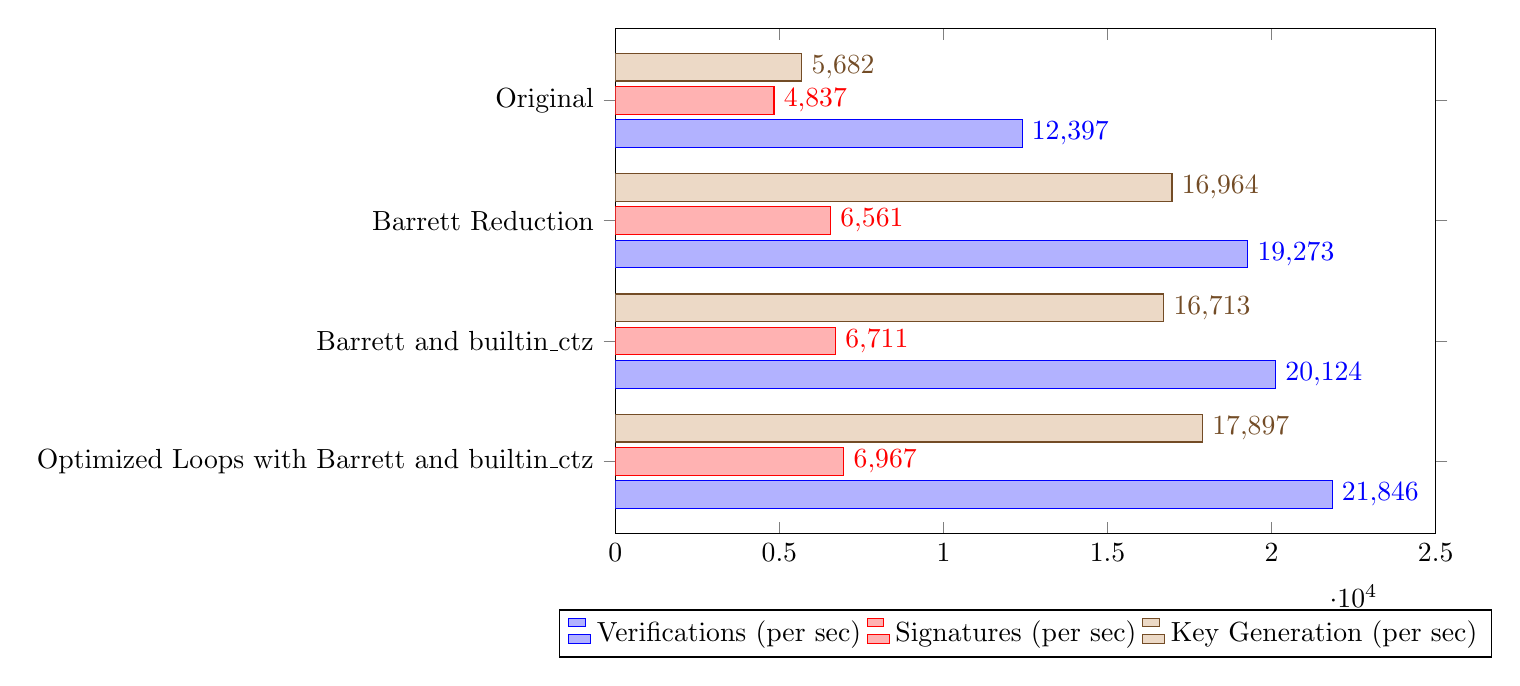
\begin{tikzpicture}
\begin{axis}[xbar, xmin=0, xmax=25000, xtick={0,5000,10000,15000,20000,25000}, ytick=data, symbolic y coords={Optimized Loops with Barrett and builtin\_ctz, Barrett and builtin\_ctz, Barrett Reduction, Original}, enlarge y limits=0.2, y tick label style={/pgf/number format/1000 sep=}, nodes near coords, nodes near coords align={horizontal}, legend style={at={(0.5,-0.15)},anchor=north,legend columns=-1},]
\addplot coordinates {(21846,Optimized Loops with Barrett and builtin\_ctz) (20124,Barrett and builtin\_ctz) (19273,Barrett Reduction) (12397,Original)};
\addplot coordinates {(6967,Optimized Loops with Barrett and builtin\_ctz) (6711,Barrett and builtin\_ctz) (6561,Barrett Reduction) (4837,Original)};
\addplot coordinates {(17897,Optimized Loops with Barrett and builtin\_ctz) (16713,Barrett and builtin\_ctz) (16964,Barrett Reduction) (5682,Original)};
\legend{Verifications (per sec), Signatures (per sec), Key Generation (per sec)}
\end{axis}
\end{tikzpicture}
\caption{Performance gains from optimised NTT loops [Intel i7 6700 CPU @ 3.4GHz]}
\label{fig:bliss_b_optimised_ntt}
\end{figure}

  \item The NTT roots of unity tables are stored using the minimum bit width type required. When these coefficients are used in multiplication routines they are typically cast to an int64\_t or a double, and within the loop operations of the NTT/INTT they are read infrequently relative to other variables. Therefore using the minimal storage type reduces the memory use within the image whilst having no impact on performance.
\end{itemize}

\subsubsection{CSPRNG}
\begin{itemize}

  \item A range of PRNG's are provided by the SAFEcrypto library: ISAAC \cite{issac}, KISS \cite{kiss}, AES-PRNG (utilizes Brian Gladman's AES \cite{aes_gladman}) and CHACHA20-CSPRNG \cite{chacha20_csprng}.
  \item A functional test of the various CSPRNG options was used to determine their relative performance - the results are shown in Figure \ref{fig:hash_mbyte_per_sec}.

\pgfplotsset{compat=1.13,width=10cm,height=9cm}
\begin{figure}[ht!]
\centering
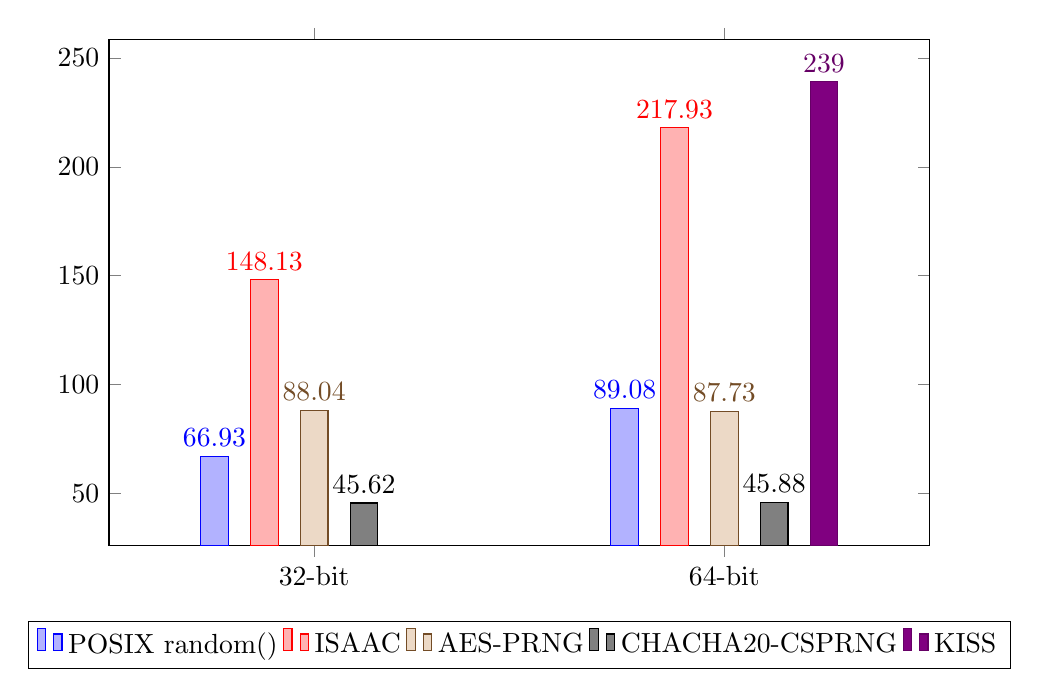
\begin{tikzpicture}
\begin{axis}[ybar=8pt, xtick=data, enlarge x limits=0.5, symbolic x coords={32-bit, 64-bit}, x tick label style={/pgf/number format/1000 sep=}, nodes near coords, nodes near coords align={vertical}, legend style={at={(.5,-0.15)},anchor=north,legend columns=-1}]
\addplot coordinates {(32-bit, 66.933) (64-bit, 89.083)};
\addplot coordinates {(32-bit, 148.129) (64-bit, 217.928)};
\addplot coordinates {(32-bit, 88.041) (64-bit, 87.73)};
\addplot coordinates {(32-bit, 45.615) (64-bit, 45.882)};
\addplot coordinates {(64-bit, 239.004)};
\legend{POSIX random(), ISAAC, AES-PRNG, CHACHA20-CSPRNG, KISS}
\end{axis}
\end{tikzpicture}
\caption{Performance of various CSPRNG schemes in MByte/sec [Intel i7 6700 CPU @ 3.4GHz]}
\label{fig:hash_mbyte_per_sec}
\end{figure}

\noindent \textbf{NOTE: KISS is 64-bit only, we probably need to implement the 32-bit version for comparison purposes.}

\item The performance of BLISS-B with no entropy coding whilst using a range of CSPRNG's is shown in Figure \ref{fig:bliss_b_csprng_comparison}. As expected there is no real difference in improvement for the verification operation as it requires no random number generation. The higher performance of KISS and ISAAC translates to higher performance within BLISS-B, with both CSPRNG's offering very similar performance.

\pgfplotsset{compat=1.13,width=15cm,height=10cm}
\begin{figure}[ht!]
\centering
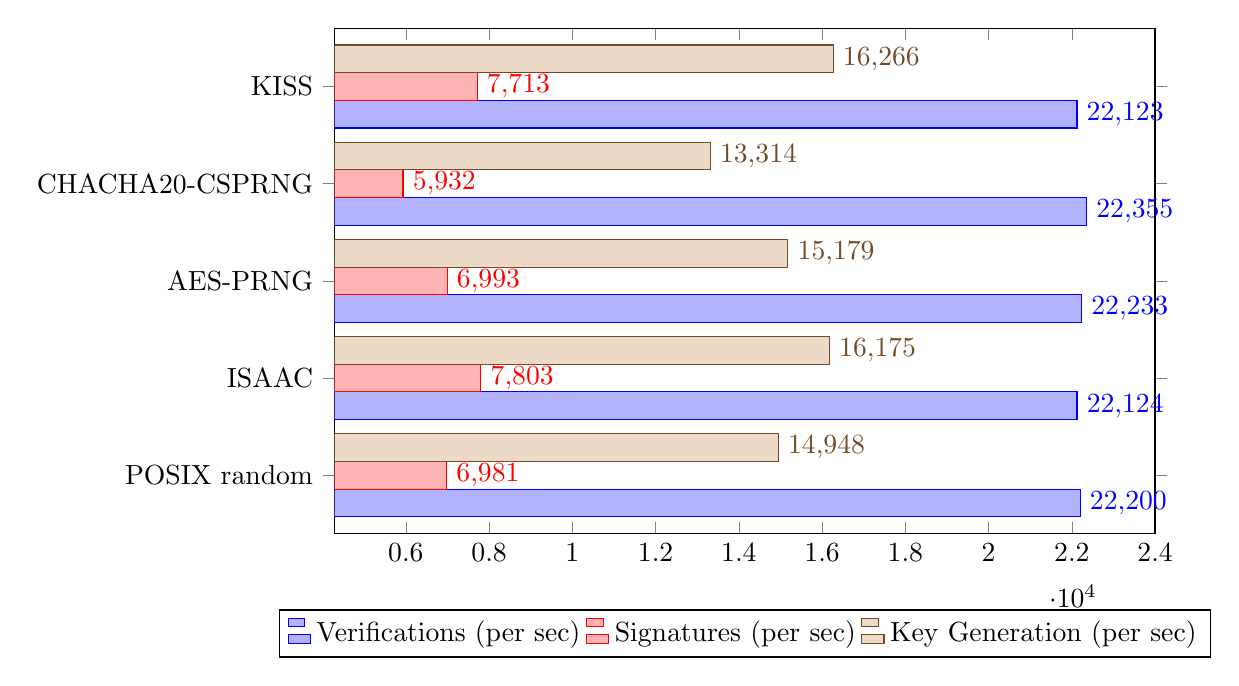
\begin{tikzpicture}
\begin{axis}[xbar=0pt, ytick=data, enlarge y limits=0.15, symbolic y coords={POSIX random, ISAAC, AES-PRNG, CHACHA20-CSPRNG, KISS}, y tick label style={/pgf/number format/1000 sep=}, nodes near coords, nodes near coords align={horizontal}, legend style={at={(.5,-0.15)},anchor=north,legend columns=-1}]
\addplot coordinates {(22200,POSIX random) (22124,ISAAC) (22233,AES-PRNG) (22355,CHACHA20-CSPRNG) (22123,KISS)};
\addplot coordinates {(6981,POSIX random) (7803,ISAAC) (6993,AES-PRNG) (5932,CHACHA20-CSPRNG) (7713,KISS)};
\addplot coordinates {(14948,POSIX random) (16175,ISAAC) (15179,AES-PRNG) (13314,CHACHA20-CSPRNG) (16266,KISS)};
\legend{Verifications (per sec), Signatures (per sec), Key Generation (per sec)}
\end{axis}
\end{tikzpicture}
\caption{Performance of various CSPRNG schemes in BLISS-B-IV [Intel i7 6700 CPU @ 3.4GHz]}
\label{fig:bliss_b_csprng_comparison}
\end{figure}

\end{itemize}


\clearpage
\subsection{Verification}

\begin{itemize}
\item Reject if $||(z_1 | 2^d . z_2)||_2 > B_2$
\item Reject if $||(z_1 | 2^d . z_2)||_\infty > B_2$
\item Accept if $c = H(\lfloor a_1 . z_1 + q . c \rceil_d + z_2 mod p, \mu)$
\end{itemize}

Verification utilises some of the same functions as signing (NTT, Hashing, checking the signature norms) so achieves the same gains when these are improved.

\begin{itemize}
\item There are some operations that require a polynomial to be reduced using \textit{2q} or \textit{p} rather than \textit{q}. These have also been accelerated using Barrett and Floating Point reduction techniques, taking care to structure the code such that automatic vectorisation is enabled by the compiler.
\end{itemize}



\subsection{General Performance Improvements}

\begin{itemize}
\item Intermediate storage is achieved using heap memory allocated when the schemes call the \textit{create()} functions. This memory is released when the scheme is destroyed. This means that when any cryptographic functions are called there is no dynamic memory allocation or static memory used to store intermediate variables.
\item Integer and floating point types of 32-bit or larger are preferred on x86/AMD64 as the compiler can exploit SIMD/AVX auto-vectorization. This compiler optimization is to be investigated further for other microprocessor architectures.
\end{itemize}


\subsection{Summary}

The original hilabliss/BLZZRD implementations of BLISS are reference designs used to show the algorithms and functional operation of the signature scheme; as such they are intended to be non-optimal.

We have shown that the use of a Binary Arithmetic Coder within BLZZRD is sub-optimal in terms of performance, both as a Gaussian Sampler and an entropy coder. Huffman is significantly faster, whilct as a Gaussian Sampler it is statistically poor.

Also, hilabliss/BLZZRD and many other lattice-based cryptographic schemes are using SHA-3 as a hash function when implementing a random oracle. It is shown that this is a poor choice in terms of performance if not security. Therefore it is strongly suggested that a more optimal choice of hash would be SHA-2 or BLAKE2-B, both are standardized and strong hash functions in line with SHA-3.

The performance gains that have been achieved are summarised in Figures \ref{fig:bliss_b_no_entropy_comparison} and \ref{fig:bliss_b_entropy_comparison}. In this diagram the original algorithm is shown in comparison to (a) a version in which the NTT's and modular reduction have been optimised and (b) a version in which the the BLISS-B algorithm has been fully optimised with the addition of the ISAAC as a CSPRNG and BLAKE2 as a hash function. In all of these implementations entropy coding is disabled.

\noindent \textbf{I hope to add a multithreaded version in which the CSPRNG and Gaussian Sampler have been placed into worker threads which should be significantly faster again, even if it is cheating!}

\pgfplotsset{compat=1.13,width=12cm,height=8cm}
\begin{figure}[ht!]
\centering
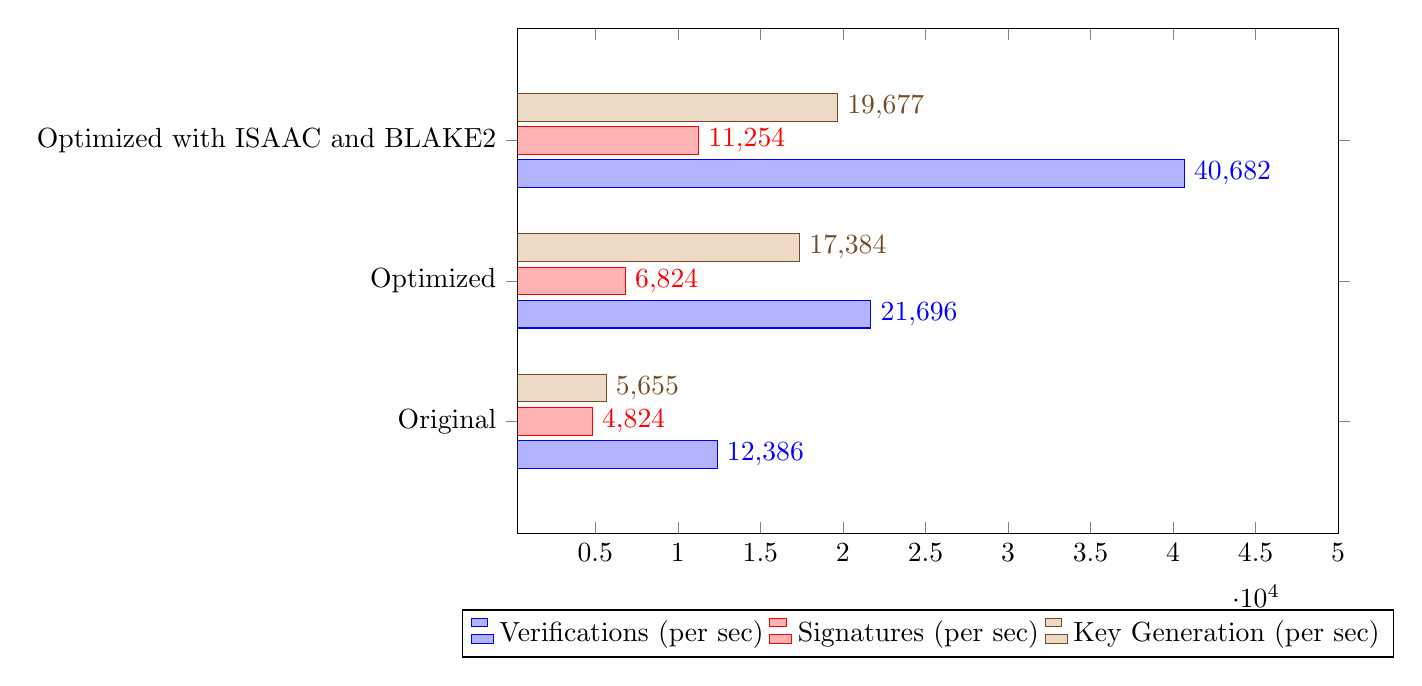
\begin{tikzpicture}
\begin{axis}[xbar=2pt, xmax=50000, ytick=data, enlarge y limits=0.4, symbolic y coords={Original, Optimized, Optimized with ISAAC and BLAKE2}, y tick label style={/pgf/number format/1000 sep=}, nodes near coords, nodes near coords align={horizontal}, legend style={at={(.5,-0.15)},anchor=north,legend columns=-1}]
\addplot coordinates {(40682,Optimized with ISAAC and BLAKE2) (21696,Optimized) (12386,Original)};
\addplot coordinates {(11254,Optimized with ISAAC and BLAKE2) (6824,Optimized) (4824,Original)};
\addplot coordinates {(19677,Optimized with ISAAC and BLAKE2) (17384,Optimized) (5655,Original)};
\legend{Verifications (per sec), Signatures (per sec), Key Generation (per sec)}
\end{axis}
\end{tikzpicture}
\caption{Performance of SAFEcrypto BLISS-B-IV with no entropy coding [Intel i7 6700 CPU @ 3.4GHz]}
\label{fig:bliss_b_no_entropy_comparison}
\end{figure}

\pgfplotsset{compat=1.13,width=12cm,height=8cm}
\begin{figure}[ht!]
\centering
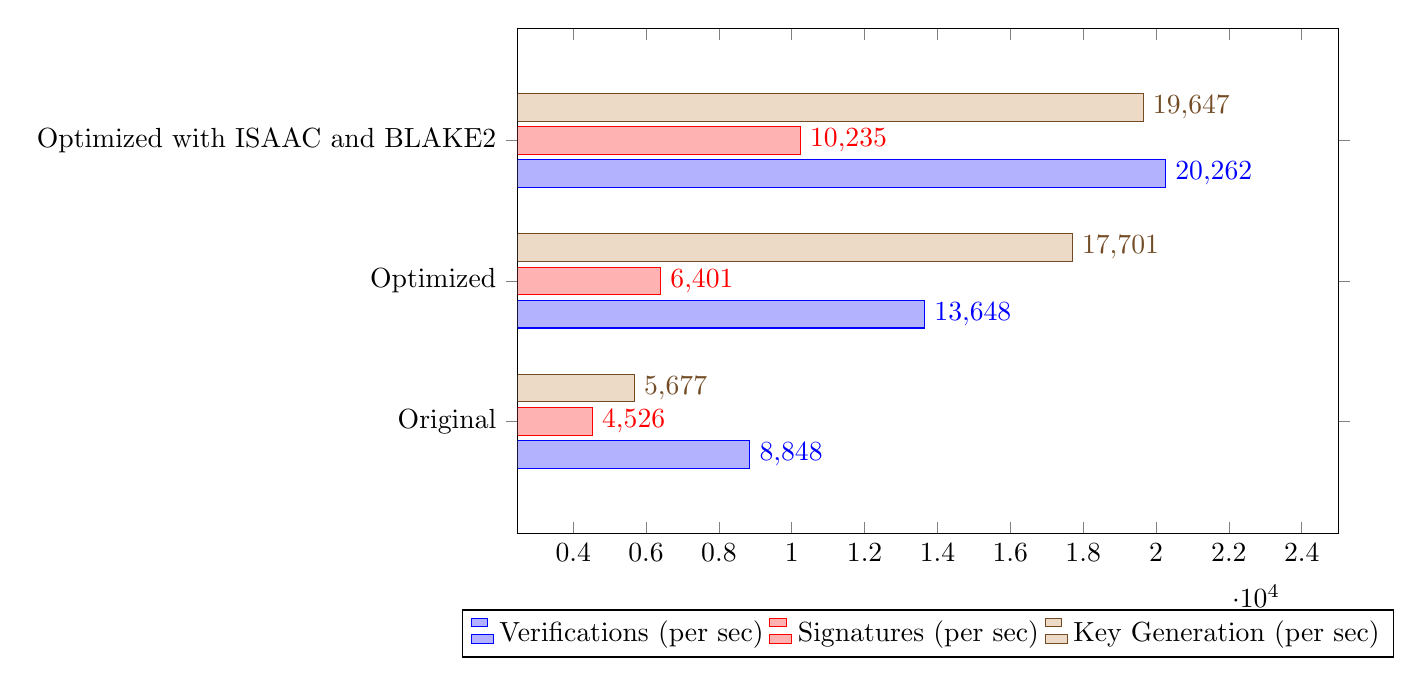
\begin{tikzpicture}
\begin{axis}[xbar=2pt, xmax=25000, ytick=data, enlarge y limits=0.4, symbolic y coords={Original, Optimized, Optimized with ISAAC and BLAKE2}, y tick label style={/pgf/number format/1000 sep=}, nodes near coords, nodes near coords align={horizontal}, legend style={at={(.5,-0.15)},anchor=north,legend columns=-1}]
\addplot coordinates {(20262,Optimized with ISAAC and BLAKE2) (13648,Optimized) (8848,Original)};
\addplot coordinates {(10235,Optimized with ISAAC and BLAKE2) (6401,Optimized) (4526,Original)};
\addplot coordinates {(19647,Optimized with ISAAC and BLAKE2) (17701,Optimized) (5677,Original)};
\legend{Verifications (per sec), Signatures (per sec), Key Generation (per sec)}
\end{axis}
\end{tikzpicture}

\textbf{[Put comparisons to other implementations of BLISS-B in here as it is compatible.]}
\caption{Performance of SAFEcrypto BLISS-B-IV with Huffman compression [Intel i7 6700 CPU @ 3.4GHz]}
\label{fig:bliss_b_entropy_comparison}
\end{figure}


\clearpage
In Figure \ref{fig:bliss_b_comparison} the original implementation of BLZZRD \cite{markku_blzzrd} is compared to a compatible implementation created using the SAFEcrypto library (i.e. SHA-3, Binary Arithmetic Coding and Blinding countermeasures). Verification is shown to be approximately 14\% slower using the SAFEcrypto library which can be attributed to the poor performance of the BAC decoder (\textit{some more effort could be exercised in trying to improve this}). However, the signature performance is approximately 25\% faster whilst key generation is significantly faster by 330\%.

A higher performance version of BLZZRD, here called \textit{BLZZRD+}, has been implemented to address the poor performance associated with the BAC and hash. BLZZRD+ utilises the more efficient BLAKE2 hash function, Ziggurat Gaussian Sampling and Huffman coding, whilst maintaining blinding countermeasures. As such it gains much greater performance for signing and verifying, being approximately 250\% and 170\% faster respectively than the original BLZZRD implementation.

\textit{The paper in \cite{markku_blzzrd} quotes performance on a 2.5GHz i7 in milliseconds per operation. To scale these figures for use here they have been inverted to convert to operations per second and muliplied by $1.36$ to scale to a 3.4GHz i7.}

\pgfplotsset{compat=1.13,width=12cm,height=8cm}
\begin{figure}[ht!]
\centering
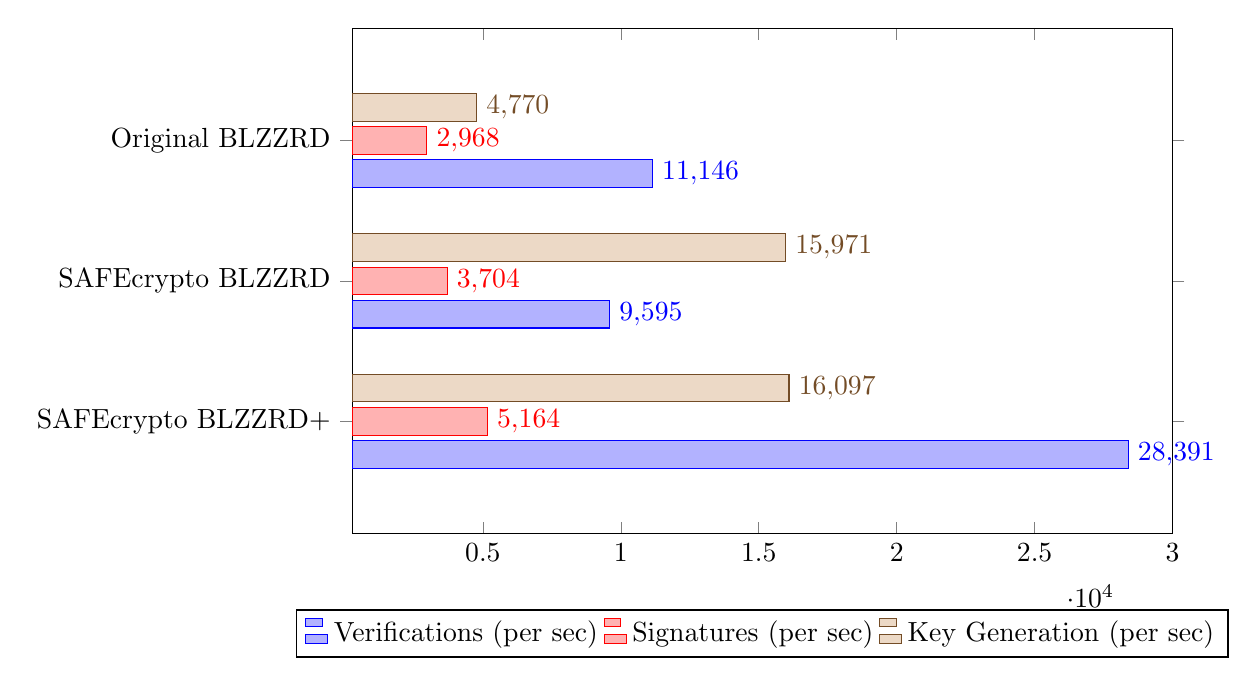
\begin{tikzpicture}
\begin{axis}[xbar=2pt, xmax=30000, ytick=data, enlarge y limits=0.4, symbolic y coords={SAFEcrypto BLZZRD+, SAFEcrypto BLZZRD, Original BLZZRD}, y tick label style={/pgf/number format/1000 sep=}, nodes near coords, nodes near coords align={horizontal}, legend style={at={(.5,-0.15)},anchor=north,legend columns=-1}]
\addplot coordinates {(28391,SAFEcrypto BLZZRD+) (9595,SAFEcrypto BLZZRD) (11146,Original BLZZRD)};
\addplot coordinates {(5164,SAFEcrypto BLZZRD+) (3704,SAFEcrypto BLZZRD) (2968,Original BLZZRD)};
\addplot coordinates {(16097,SAFEcrypto BLZZRD+) (15971,SAFEcrypto BLZZRD) (4770,Original BLZZRD)};
\legend{Verifications (per sec), Signatures (per sec), Key Generation (per sec)}
\end{axis}
\end{tikzpicture}
\caption{Performance comparison of SAFEcrypto BLZZRD-IV [Intel i7 6700 CPU @ 3.4GHz]}
\label{fig:bliss_b_comparison}
\end{figure}

